\chapter{Physics}

%-----------------------------------------------------------------
\section{Units}
\label{s:units}
\index{Units|textbf}

\index{MAD!units}
\index{Units!with MAD}
\bmad uses SI (Syst\'eme International) units as shown in
Table~\ref{t:units}.  Note that \mad uses different units. For example,
\mad's unit of Particle Energy is GeV not eV.
\begin{table}[ht]
\centering
\begin{tabular}{|l|l|} \hline
  {\em Quantity}     & {\em Units}       \\ \hline
  Angles             &    radians        \\ 
  Charge             &    Coulombs       \\
  Current            &    Amps           \\ 
  Frequency          &    Hz             \\ 
  Kick               &    radians        \\ 
  Length             &    meters         \\ 
  Magnetic Field     &    Tesla          \\ 
  Particle Energy    &    eV             \\ 
  Phase Angles (RF)  &    radians/2$\pi$ \\ 
  Voltage            &    Volts          \\ \hline
\end{tabular}
\caption{Physical units used by \bmad.}
\label{t:units}
\end{table}


%-----------------------------------------------------------------
\section{Constants}
\label{s:constants}
\index{Constants|textbf}

\index{MAD}
\bmad defines commonly used physical and mathematical constants
shown in Table~\ref{t:constants}.  All symbols use straight SI units
except for \vn{e_mass} and \vn{p_mass} which are provided for
compatibility with \mad.

\begin{table}
\centering
\begin{tabular}{|l|l|l|l|} \hline
  {\em Symbol}  & {\em Value}       & {\em Units} &  {\em Name}       \\ \hline
  pi            & 3.14159265359          &        &                   \\
  twopi         & 2 * pi                 &        &                   \\
  fourpi        & 4 * pi                 &        &                   \\
  sqrt_2        & 1.4142135623731        &        &                   \\
  m_electron    & $0.51099906 \pow{6}$   & eV     & Electron mass     \\
  m_proton      & $0.938271998 \pow{9}$  & eV     & Proton mass       \\
  c_light       & $2.99792458 \pow{8}$   & m/s    & Speed of light    \\
  r_e           & $2.8179380 \pow{-15}$  & m      & Electron radius   \\
  r_p           & $1.5346980 \pow{-18}$  & m      & Proton radius     \\
  e_charge      & $1.6021892 \pow{-19}$  & C      & Electron charge   \\
  h_planck      & $6.626196 \pow{-34}$   & J/Hz   & Planck's constant \\
  h_bar_planck  & $1.054591 \pow{-34}$   & J s    & Planck / $2\pi$   \\
  e_mass        & $0.51099906 \pow{-3}$  & GeV    & Electron mass     \\
  p_mass        & $0.938271998$          & GeV    & Proton mass       \\ \hline
\end{tabular}
\caption{Physical and mathematical constants recognized by \bmad.}
\label{t:constants}
\end{table}


%-----------------------------------------------------------------
\section{Magnetic Fields}
\label{s:fields}
\index{Magnetic fields|textbf}

Start with the assumption that the local magnetic field has no
longitudinal component (obviously this assumption does not work with,
say, a solenoid).  Following \mad, the vertical magnetic field along
the $y = 0$ axis is expanded in a Taylor series
\Begineq
  B_y(x, 0) = \sum_n B_n \, \frac{x^n}{n!}
  \label{byx0b}
\Endeq
This is not the most
general form for the magnetic field. Essentially all of the skew
components have been ignored here. Assuming that the
reference orbit is locally straight (there are correction terms if the
Reference Orbit is locally curved), the field up to $3^{rd}$ order is
\begin{alignat}{5}
  B_x &=           &&B_1 y \plus         &&B_2 \, xy       
                   && \plus && \frac{1}{6} B_3 (3x^2 y - y^3) \plus \ldots \\
  B_y &= B_0 \plus &&B_1 x + \frac{1}{2} &&B_2 (x^2 - y^2) 
                   && \plus && \frac{1}{6} B_3 (x^3 - 3x y^2) \plus \ldots
\end{alignat}
The normalized integrated multipole $K_nL$ is used when specifying magnetic
multipole components
\index{Multipole!KnL, Tn|textbf}
\Begineq
  K_nL \equiv \frac{q \, L \, B_n}{P_0}
\Endeq
$L \, B_n$ is the integrated multipole component over a length $L$,
and $P_0$ is the reference momentum. Note that $P_0/q$ is sometimes
written as $B\rho$. This is just an old notation where $\rho$ is the
bending radius of a particle with the reference energy in a field of
strength $B$. The kicks $\Delta p_x$ and $\Delta p_y$ that a
particle experiences going through a multipole field is
\begin{alignat}{5}
  \Delta p_x & = \frac{-q \, L \, B_y}{P_0} \label{pqlbp1} \\
             & = -K_0 L \;-\; 
             && K_1 L \, x \plus 
             \frac{1}{2} && K_2 L (y^2 - x^2) && \plus 
             && \frac{1}{6} K_3 L (3x y^2 - x^3) \plus \ldots 
             \nonumber \\
  \Delta p_y & = \frac{q \, L \, B_x}{P_0} \label{pqlbp2} \\
             & =     
             && K_1 L \, y \plus 
             && K_2 L \, xy && \plus 
             && \frac{1}{6} K_3L (3x^2 y - y^3) \plus \ldots \nonumber 
\end{alignat}
A positive $K_1L$ quadrupole component gives
horizontal focusing and vertical defocussing. The general form is
\begin{align}
  \Delta p_x &= \sum_{n = 0}^{\infty} \frac{K_n L}{n!} 
             \sum_{m = 0}^{\lfloor \frac{n}{2} \rfloor}
             \begin{pmatrix} n \cr 2m \end{pmatrix} \,
             (-1)^{m+1} \, x^{n-2m} \, y^{2m} \\
  \Delta p_y &= \sum_{n = 0}^{\infty} \frac{K_n L}{n!} 
             \sum_{m = 0}^{\lfloor \frac{n-1}{2} \rfloor}
             \begin{pmatrix} n \cr 2m+1 \end{pmatrix} \,
             (-1)^{m} \, x^{n-2m-1} \, y^{2m+1}
\end{align}

\index{Multipole!KnL, Tn|textbf}
So far only the normal components of the field have been
considered. If the fields associated with a particular $B_n$ multipole
component are rotated in the $(x, y)$ plane by an angle $\theta_n$, the
magnetic field at a point $(x,y)$ can be expressed in complex notation
as
\Begineq
  B_y(x,y) + i B_x(x,y) = 
    \frac{1}{n!} B_n e^{-i(n+1)\theta_n} \, e^{i n \theta} \, r^n 
  \label{bib1nb}
\Endeq
where $(r, \theta)$ are the polar coordinates of the point $(x, y)$.

\index{Multipole!an, bn|textbf}
Another representation of the magnetic field used by \bmad divides
the fields into normal $b_n$ and skew $a_n$ components. In terms of
these components the magnetic field for the $n$\Th\ order multipole is
\Begineq
  \frac{q \, L}{P_0} \, (B_y + i B_x) = (b_n + i a_n) \, (x + i y)^n
\Endeq
The conversion between $(a_n, b_n)$ and $(K_nL, \theta_n)$ is
\Begineq
  b_n + i a_n = \frac{1}{n!} \, K_nL \, e^{-i(n+1)\theta_n}
\Endeq
or
\begin{align}
  K_n L &= n! \, \sqrt{a_n^2 + b_n^2} \\
  \tan[(n+1) \theta_n] &= \frac{-a_n}{b_n}
\end{align}
To convert a normal magnet (a magnet with no skew component) into a skew
magnet (a magnet with no normal component) the magnet should be rotated
about its longitudinal axis with a rotation angle of
\Begineq
  (n+1) \theta_n = \frac{\pi}{2}
\Endeq
For example, a normal quadrupole rotated by $45^\circ$ becomes a
skew quadrupole.

\index{AB_Multipole}
\index{Radius}
When the $a_n$ and $b_n$ are associated with a physical element (as
opposed to the $a_n$ and $b_n$ associated with an \vn{AB_Multipole} element),
a measurement radius $r_0$ and a scale factor $F$ are used to scale
the $a_n$ and $b_n$ according to the formula
\Begineq
  \bigl[ a_n (\text{actual}), b_n (\text{actual}) \bigr] =
  \bigl[ a_n (\text{input}), b_n (\text{input}) \bigr] 
  \cdot F \cdot \frac{r_0^{n_\text{ref}}}{r_0^n} 
  \label{ababf}
\Endeq
$a_n(\text{input})$ and $b_n(\text{input})$ are the multipole values as given in the
lattice file. $a_n(\text{actual})$ and $b_n(\text{actual})$ are the multipole values
that are used in any simulation calculations. $r_0$ is set by the
\vn{radius} attribute of an element. $F$ and $n_\text{ref}$ are set
automatically depending upon the type of element as shown in
Table~\ref{t:ab}.

\index{AB_Multipole}
\index{Multipole}
Note that the $n = 0$ component of an \vn{AB_Multipole} or \vn{Multipole}
element rotates the reference orbit essentially acting as a zero length bend.
This is not true for multipoles that are associated with 
non-multipole elements.

\index{Kicker}
\index{Hkicker}
\index{Vkicker}
\index{Rbend}
\index{Sbend}
\index{Elseparator}
\index{Quadrupole}
\index{Solenoid}
\index{Sol_Quad}
\index{Sextupole}
\index{Octupole}
\begin{table}[ht]
\centering
\begin{tabular}{|l|l|l|} \hline
\tt
  {\em Element} & $F$                              & $n_\text{ref}$ \\ \hline
  \vn{Kicker}      & $\sqrt{{\tt Hkick}^2 + {\tt Vkick}^2}$ & 0 \\
  \vn{Hkicker}     & Kick                                   & 0 \\
  \vn{Vkicker}     & Kick                                   & 0 \\
  \vn{Rbend}       & G * L                                  & 0 \\
  \vn{Sbend}       & G * L                                  & 0 \\
  \vn{Elseparator} & $\sqrt{{\tt Hkick}^2 + {\tt Vkick}^2}$ & 0 \\
  \vn{Quadrupole}  & K1 * L                                 & 1 \\
  \vn{Solenoid}    & KS * L                                 & 1 \\
  \vn{Sol_Quad}    & K1 * L                                 & 1 \\
  \vn{Sextupole}   & K2 * L                                 & 2 \\
  \vn{Octupole}    & K3 * L                                 & 3 \\ \hline
\end{tabular}
\caption{$F$ and $n_\text{ref}$ for various elements.}
\label{t:ab}
\end{table}

%-----------------------------------------------------------------
\section{Taylor Maps}
\label{s:taylor_phys}
\index{Taylor map|textbf}

A transport map ${\cal M}: {\cal R}^6 \rightarrow {\cal R}^6$ through
an element or a section of a lattice is a function that maps the
starting phase space coordinates $\Bf r(\In)$ to the ending
coordinates $\Bf r(\Out)$
\begin{equation}
  \Bf r(\Out) = {\cal M} \, \Bf r(\In)
\end{equation}
${\cal M}$ is made up of six functions ${\cal M}_i: {\cal R}^6
 \rightarrow {\cal R}$. Each of these functions maps to one of the $r(\Out)$
coordinates. These functions can be expanded in a Taylor
series and truncated at some order. Each Taylor series is in the form
\Begineq
  r_i(\Out) = \sum_{j = 1}^N \, C_{ij} \, \prod_{k = 1}^6 \, r_k^{e_{ijk}}(\In)
  \label{rcr}
\Endeq
Where the $C_{ij}$ are coefficients and the $e_{ijk}$ are integer exponents.
The order of the map is
\Begineq
  \mbox{order} = \max_{i,j} \left( \sum_{k = 1}^6 e_{ijk} \right)
\Endeq

The standard \bmad routine for printing a Taylor map might produce something 
like this: 
\begin{example}
   Taylor Terms:
    Out     Coef              Exponents           Order        Reference
   ---------------------------------------------------
      1:     -0.600000000000  0  0  0  0  0  0        0       0.200000000
      1:      1.000000000000  1  0  0  0  0  0        1
      1:      0.145000000000  2  0  0  0  0  0        2
   ---------------------------------------------------
      2:     -0.185000000000  0  0  0  0  0  0        0       0.000000000
      2:      1.300000000000  0  1  0  0  0  0        1
      2:      3.800000000000  2  0  0  0  0  1        3
   ---------------------------------------------------
      3:      1.000000000000  0  0  1  0  0  0        1       0.100000000
      3:      1.600000000000  0  0  0  1  0  0        1
      3:    -11.138187077310  1  0  1  0  0  0        2
   ---------------------------------------------------
      4:      1.000000000000  0  0  0  1  0  0        1       0.000000000
   ---------------------------------------------------
      5:      0.000000000000  0  0  0  0  0  0        0       0.000000000
      5:      0.000001480008  0  1  0  0  0  0        1
      5:      1.000000000000  0  0  0  0  1  0        1
      5:      0.000000000003  0  0  0  0  0  1        1
      5:      0.000000000003  2  0  0  0  0  0        2
   ---------------------------------------------------
      6:      1.000000000000  0  0  0  0  0  1        1       0.000000000
\end{example}
Each line in the example represents a single taylor term. The Taylor
terms are grouped into 6 Taylor series, one each output phase space
coordinate.  The first column in the example, labeled ``out'',
(corresponding to the $i$ index in \Eq{rcr}) indicates the Taylor
series: $1 = x(out)$, $2 = p_x(out)$, etc. The 6 exponent columns give
the $e_{ijk}$ of \Eq{rcr}. In this example, the second Taylor series
(\vn{out} = 2), when expressed as a formula, would read:
\Begineq
  p_x(out) = -0.185 + 1.3 \, p_x(in) + 3.8 \, x^2(in) \, p_z(in)
\Endeq

\index{Taylor map!reference coordinates}
The reference column in the above example shows the input coordinates around
which the Taylor map is calculated. In this case, the reference
coordinates where 
\Begineq
  (x, p_x, y, p_y, z, p_z)_{ref} = (0.2, 0, 0.1, 0, 0, 0, 0)
\Endeq
The choice of the reference point will affect the values of the
coefficients of the Taylor map. For example, suppose that the exact
map through an element looks like
\Begineq
  x(out) = A \, \sin(k \, x(in))
\Endeq
Then a Taylor map to 1\St order is
\Begineq
  x(out) = c_0 + c_1 \, x(in)
\Endeq
where
\begin{align}
  c_1 &= A \, k \, \cos(k \, x_{\mbox{ref}}) \\
  c_0 &= A \, \sin(k \, x_{\mbox{ref}}) - c_1 \, x_{\mbox{ref}} \nonumber
\end{align}
Notice that once the coefficient values are determined the reference
point does not play any role when the Taylor map is evaluated to
determine the output coordinates as a function of the input
coordinates.

\index{Taylor map!feed-down}
Of importance in working with Taylor maps is the concept of
\vn{feed-down}.  This is best explained with an example. To keep the
example simple, the discussion is limited to one phase space
dimension so that the Taylor maps are a single Taylor series. Take the
map $M_1$ from point 0 to point 1 to be
\Begineq
  M_1: x_1 = x_0 + 2
  \label{xx2}
\Endeq
and the map $M_2$ from point 1 to point 2 to be
\Begineq
  M_2: x_2 = x_1^2 + 3 \, x_1
  \label{xx3x}
\Endeq
Then concatenating the maps to form the map $M_3$ from point 0 to point 2
gives
\Begineq
  M_3: x_2 = (x_0 + 2)^2 + 3 (x_0 + 2) = x_0^2 + 7 \, x_0 + 10
  \label{xx23x2}
\Endeq
However if we are evaluating our maps to only 1\St order the map $M_2$
becomes
\Begineq
  M_2: x_2 = 3 \, x_1
\Endeq
and concatenating the maps now gives
\Begineq
  M_3: x_2 = 3 (x_0 + 2) = 3 \, x_0 + 6
  \label{x3x23}
\Endeq
Comparing this to \Eq{xx23x2} shows that by neglecting the 2\Nd order
term in \Eq{xx3x} leads to 0\Th and 1\St order errors in
\Eq{x3x23}. These errors can be traced to the finite 0\Th order term in
\Eq{xx2}. This is the principal of feed--down: Given $M_3$ which is a map
produced from the concatenation of two other maps, $M_1$, and $M_2$
\Begineq
  M_3 = M_2(M_1)
\Endeq
Then if $M_1$ and $M_2$ are correct to n\Th order, $M_3$ will also be
correct to n\Th order as long as $M_1$ has no constant (0\Th order)
term. [Notice that a constant term in $M_2$ does not affect the
argument.]  What happens if we know there are constant terms in our
maps? One possibility is to go to a coordinate system where the
constant terms vanish. In the above example that would mean using the
coordinate $\widetilde x_0$ at point 0 given by
\Begineq
  \widetilde x_0 = x_0 + 2
\Endeq
\index{Symplectic integration}
The other possibility is to use symplectic integration. By its nature,
symplectic integration never has problems with feed--down.

The subject of symplectic integration is too large to be covered in
this guide. The reader is referred to the book ``Beam Dynamics: A New
Attitude and Framework'' by Etienne Forest\cite{b:forest}. A brief
synopsis: Symplectic integration uses as input 1) The Hamiltonian that
defines the equations of motion, and 2) a Taylor map $M_1$ from point 0 to
point 1. Symplectic integration from point 1 to point 2 produces a
Taylor map $M_3$ from point 0 to point 2. Symplectic integration can
produce maps to arbitrary order. In any practical application the
order $n$ of the final map is specified and in the integration
procedure all terms of order higher than $n$ are ignored. If one is
just interested in knowing the final coordinates of a particle at
point 2 given the initial coordinates at point 1 then $M_1$ is just
the constant map
\Begineq
  M_1: x_1 = c_i
\Endeq
where $c_i$ is the initial starting point. The order of the
integration is set to 0 so that all non--constant terms are
ignored. The final map is also just a constant map
\Begineq
  M_3: x_2 = c_f
\Endeq
If the map from point 1 to point 2 is desired then the map $M_1$ is
just set to the identity map
\Begineq
  M_1: x_1 = x_0
\Endeq
In general it is impossible to exactly integrate any non--linear
system. In practice, the symplectic integration is achieved by slicing
the interval between point 1 and point 2 into a number of (generally
equally spaced) slices. The integration is performed, slice step by
slice step. This is analogous to integrating a function by evaluating
the function at a number of points. Using more slices gives better
results but slows down the calculation. The speed and accuracy of the
calculation is determined by the number of slices and the \vn{order}
of the integrator. The concept of integrator order can best be
understood by analogy by considering the trapezoidal rule for
integrating a function of one variable:
\Begineq
  \int_{y_a}^{y_b} f(y) \, dy = 
  h \left[ \frac{1}{2} f(y_a) + \frac{1}{2} f(y_b) \right] +
  o(h^3 \, f^{(2)})
\Endeq
In the formula $h = y_b - y_a$ is the slice width. $0(h^3 \, f^{(2)})$
means that the error of the trapezoidal rule scales as the second
derivative of $f$. Since the error scales as $f^{(2)}$ this is an
example of a second order integrator. To integrate a function between
points $y_1$ and $y_N$ we slice the interval at points $y_2 \ldots y_{N-1}$
and apply the trapezoidal rule to each interval. Examples of higher
order integrators can be found, for example, in Numerical
Recipes\cite{b:nr}. The concept of integrator order in symplectic
integration is analogous. 

The optimum number of slices is determined by the smallest number that
gives an acceptable error. Integrators of higher order will generally
need a smaller number of slices to achieve a given accuracy. However,
since integrators of higher order take more time per slice step, and
since it is computation time and not number of slices which is
important, only a measurement of error and calculation time as a
function of slice number and integrator order will unambiguously give
the optimum integrator order and slice width.  In doing a timing test
it must be remembered that since the magnitude of any non-linearities
will depend upon position, the integration error will be dependent
upon the starting map $M_1$. For example, \bmad has integrators of
order 2, 4, and 6. To test them, timing tests were performed for some
wiggler elements (which have strong nonlinearities) and it was found
that in this case the 2\Nd order integrator gave the fastest computation 
time for a given accuracy.

%-----------------------------------------------------------------
\section{Symplectification}
\label{s:symp_method}
\index{Symplectic!symplectification}

If the evolution of a system can be described using a Hamiltonian then
it can be shown that the linear part of any transport map (the Jacobian)
must obey the symplectic condition. If a matrix $\Bf M$ is not symplectic,
Healy\cite{b:healy} has provided an elegant method for finding a symplectic 
matrix that is ``close'' to $\Bf M$. The procedure is as follows:
From $\Bf M$ a matrix $\bV$ is formed via
\begin{equation}
  \bV = \Bf S (\Bf I - \Bf M)(\Bf I + \Bf M)^{-1} 
  \label{e:vsimi}
\end{equation}
where $\Bf S$ is the matrix
\Begineq
  \Bf S = 
  \begin{pmatrix} 
      0 &  1 &  0 &  0 &  0 &  0 \cr
     -1 &  0 &  0 &  0 &  0 &  0 \cr
      0 &  0 &  0 &  1 &  0 &  0 \cr
      0 &  0 & -1 &  0 &  0 &  0 \cr
      0 &  0 &  0 &  0 &  0 & -1 \cr
      0 &  0 &  0 &  0 & -1 &  0 \cr
  \end{pmatrix}
  \label{s0100}
\Endeq
$\bV$ is symmetric if and only if $\Bf M$ is symplectic. In any case,
a symmetric matrix $\Bf W$ near $\bV$ can be
formed via
\begin{equation}
  \Bf W = \frac{\bV + \bV^t}{2}
\end{equation}
A symplectic matrix $\Bf F$ is now obtained by inverting \eq{e:vsimi}
\Begineq
  \Bf F = (\Bf I + \Bf S \Bf W) (\Bf I - \Bf S \Bf W)^{-1}
\Endeq

%-----------------------------------------------------------------
\section{LINAC Accelerating Cavities (Lcavity)}
\label{s:lcav_phys}

The transverse trajectory through an \vn{Lcavity} is modeled using equations
developed by Rosenzweig and Serafini\cite{b:rosenzweig} with
\Begineqs
  b_0 &= 1 \CRNO
  b_{-1} &= 1 \nonumber
\Endeqs
and all other $b_n$ set to zero.

The transport through the body (R\&S Eq.~(9)) has been modified to give the 
correct phase-space area at non ultra-relativistic energies:
\Begineq
  \begin{pmatrix}
    x \\ 
    x'
  \end{pmatrix}_f = 
  \begin{pmatrix}
    m_{11}                      & \beta_i \, m_{12} \\
    \frac{1}{\beta_f} \, m_{21} & \frac{\beta_i}{\beta_f} \, m_{22} 
  \end{pmatrix}
  \,
  \begin{pmatrix}
    x \\ 
    x'
  \end{pmatrix}_i
\Endeq
where the $m_{ij}$ are the matrix elements from R\&S Eq.~(9) and the 
$\beta$ are the standard relativistic factors. With this, the determinate 
of the matrix is $\beta_i \, \gamma_i / \beta_f \, \gamma_f$.

The change in $z$ going through a cavity is calculated by first calculating the particle
transit time $\Delta t$
\begin{align}
  c \, \Delta t &= \int_0^l \!\! ds \, c \, \beta(s) \CRNO
  &= \int_0^l \!\! ds \, \frac{E}{\sqrt{E^2 - (mc^2)^2}} \\
  &= \frac{c \, P_{z2} - c \, P_{z1}}{G} \nonumber
\end{align}
where it has been assumed that the accelerating gradient $G$ is
constant through the cavity. In this equation $\beta = v / c$, $E$ is
the energy, and $P_{z2}$ and $P_{z1}$ are the entrance and exit
momenta. Using \Eq{zbctt}, the change in $z$ is thus
\Begineq
  z_2 = frac{\beta_2}{\beta_1} \, z_1 - 
  \beta_2 \, 
  \left(
  \frac{c \, P_{z2} - c \, P_{z1}}{G} - 
  \frac{c \, \BAR P_{z2} - c \, \BAR P_{z1}}{\BAR G}
  \right)
\Endeq
where $\BAR P$ and $\BAR G$ are the momentum and gradiant of the
reference particle.


%-----------------------------------------------------------------
\section{Wigglers}
\label{s:wiggler_phys}

\index{Wiggler}
As discussed in \sref{s:wiggler}, \bmad \vn{Wiggler} elements are
split into two classes: map type and periodic type. The map type
\vn{Wigglers} are modeled using the method of Sagan, Crittenden, and
Rubin\cite{b:wiggler}. In this model the magnetic field is written as
a sum of terms $B_i$
\Begineq
  B(x,y,z) = \sum_i B_i(x, y, z; C, k_x, k_y, k_z, \phi_z)
\Endeq 
Each term $B_i$ is specified using five numbers: 
$(C, k_x, k_y, k_z, \phi_z)$. A term can take one of three forms: The first
form is
\begin{alignat}{4}
  B_x &= -&C &\dfrac{k_x}{k_y} & \sin(\kxx) \sinh(\kyy) \cos(\ksss) \CRNEG
  B_y &=  &C &                 & \cos(\kxx) \cosh(\kyy) \cos(\ksss) \CRNEG
  B_s &= -&C &\dfrac{k_s}{k_y} & \cos(\kxx) \sinh(\kyy) \sin(\ksss) \CRneg
  & \makebox[1pt][l]{with $k_y^2 = k_x^2 + k_s^2$ .} &&&  \label{f1}
\end{alignat}
The second form is
\begin{alignat}{4}
  B_x &=  &C &\dfrac{k_x}{k_y} & \sinh(\kxx) \sinh(\kyy) \cos(\ksss) \CRNEG
  B_y &=  &C &                 & \cosh(\kxx) \cosh(\kyy) \cos(\ksss) \CRNEG
  B_s &= -&C &\dfrac{k_s}{k_y} & \cosh(\kxx) \sinh(\kyy) \sin(\ksss) \CRneg
  & \makebox[1pt][l]{with $k_y^2 = k_s^2 - k_x^2$ ,} &&&  \label{f2}
\end{alignat}
The third form is
\begin{alignat}{4}
  B_x &=  &C &\dfrac{k_x}{k_y} & \sinh(\kxx) \sin(\kyy) \cos(\ksss) \CRNEG
  B_y &=  &C &                 & \cosh(\kxx) \cos(\kyy) \cos(\ksss) \CRNEG
  B_s &= -&C &\dfrac{k_s}{k_y} & \cosh(\kxx) \sin(\kyy) \sin(\ksss) \CRneg
  & \makebox[1pt][l]{with $k_y^2 = k_x^2 - k_s^2$ .} &&& \label{f3}
\end{alignat}
The relationship between $k_x$, $k_y$, and $k_z$ ensures that
Maxwell's equations are satisfied. Since the field is given by
analytic equations, Lie algebraic techniques can be use to construct
Taylor maps to arbitrary order.

``Periodic type'' wigglers use a simplified model where the magnetic
field components are
\begin{alignat}{1}
  B_y &= \hphantom{-} B_{\max} \, \cosh(k_z \, y) \, \cos(k_z \, z) \CRNO
  B_z &= -B_{\max} \, \sinh(k_z \, y) \, \sin(k_z \, z) 
\end{alignat}
where $B_{\max}$ is the maximum field on the centerline and $k$ is
given in terms of the pole length (\vn{l_pole}) by
\Begineq
  k_z = \frac{\pi}{l_{\mbox{pole}}}
\Endeq
This type of wiggler has infinitely wide poles. With
\vn{bmad_standard} tracking and transfer matrix calculations the
vertical focusing is assumed small so averaged over a period the
horizontal motion looks like a drift and the vertical motion is
modeled as a combination focusing quadrupole and focusing octupole
giving a kick\cite{b:corbett}
\Begineq
  \frac{dp_y}{ds} = k_1 \left( y + \frac{2}{3} \, k_z^2 \, y^3 \right)
\Endeq
where
\begin{alignat}{1}
  k_1 &= \frac{-1}{2} \, \left( \frac{c \, B_{\max}}{P_0 \, (1 + p_z)} \right)^2 
\end{alignat}
with $k_1$ being the linear focusing constant. For radiation
calculations the true horizontal trajectory with $y = 0$ is needed
\Begineq
  x = \frac{\sqrt{2 \, |k_1|}}{k_z^2} \, \cos (k_z \, z)
\Endeq

%-----------------------------------------------------------------
\section{Synchrotron Radiation Damping and Excitation}
\label{s:radiation}
\index{Synchrotron radiation!damping and excitation|textbf}

Emission of synchrotron radiation by a particle can be decomposed into
two parts. The deterministic average radiation emitted produces damping
while the stochastic fluctuating part produces excitation\cite{b:jowett}.

The treatment of radiation damping by \bmad essentially follows \mad.
The average change in energy $\Delta E$ of a particle going through a
section of magnet due to synchrotron radiation is
\Begineq
  \frac{\Delta E}{E_0} = -k_d \, (1 + p_z)
\Endeq
where
\Begineq
  k_d \equiv \frac{2 \, r_e}{3} \, \gamma_0^3 \, \ave{g_0^2} \, L_p \,  
  (1 + p_z)
  \label{k2r3g}
\Endeq
$r_e$ is the classical electron radius, $L_p$ is the actual path
length, $\gamma_0$ is the energy factor of an on-energy particle, $1/g_0$
is the bending radius of an on--energy particle, and $\ave{g_0^2}$ is an
average of $g_0^2$ over the actual path.

The energy lost is given by
\Begineq
  \frac{\Delta E}{E_0} = -k_f \, (1 + p_z)
\Endeq
where
\Begineq
  k_f \equiv \left( \frac{55 \, r_e \, \hbar \, c}{24 \, \sqrt{3} \, m_e} \, 
  L_p \, \gamma_0^5 \ave{g_0^3} \right)^{1/2} \, (1 + p_z) \, \xi
  \label{k55rh}
\Endeq
$\xi$ is a Gaussian distributed random number with unit sigma and zero mean.

Using \Eqs{k2r3g} and \eq{k55rh} The total change in $p_z$ can be written as
\Begineq
  \Delta p_z = \frac{\Delta E}{E_0} = -k_E \, (1 + p_z)
\Endeq
where
\Begineq
  k_E = k_d + k_f
\Endeq
Since the radiation is emitted in the forward direction the angles
$x'$ and $y'$ are invariant which leads to the following equations for
the changes in $p_x$ and $p_y$
\begin{align}
  \Delta p_x &= -k_E \, p_x \CRNO
  \Delta p_y &= -k_E \, p_y 
\end{align}

The above formalism does not take into account the fact that radiation is 
emitted with a $1/\gamma$ angular distribution. This means that the calculated
vertical emittance for a lattice with
bends only in the horizontal plane and without any coupling elements such as
skew quadrupoles will be zero. Typically, in practice, the vertical emittance
will be dominated by coupling so this approximation is generally a good one.

%-----------------------------------------------------------------
\section{Coupling and Normal Modes}
\label{s:coupling}
\index{Normal Mode!Coupling}

The coupling formalism used by \bmad is taken from the paper of Sagan
and Rubin\cite{b:coupling}. The main equations are reproduced here.  A
one--turn map $\bfT(s)$ for the transverse two--dimensional phase space
$\bfx = (x, x', y, y')$ starting and ending at some point $s$ can be
written as
  \Begineq
    \bfT = \bfV \, \bfU \, \bfV\inv 
    , \label{tvuv}
  \Endeq 
where $\bfV$ is symplectic, and $\bfU$ is of the form
  \Begineq
    \bfU = 
    \begin{pmatrix}
      \bfA & \Bf0 \cr 
      \Bf0 & \bfB \cr
    \end{pmatrix}
    . \label{ua00b}
  \Endeq
\index{Normal Mode!a--mode}
\index{Normal Mode!b--mode}
Since $\bfU$ is uncoupled the standard Twiss analysis can be
performed on the matrices $\bfA$ and $\bfB$. The normal modes
are labeled $a$ and $b$ and if the one--turn matrix $\bfT$ is
uncoupled then $a$ corresponds to the horizontal mode and $b$
corresponds to the vertical mode. 

$\bfV$ is written in the form
  \Begineq
    \bfV = 
    \begin{pmatrix}
        \gamma \bfI & \bfC \cr 
        -\bfC^+     & \gamma \bfI \cr
    \end{pmatrix}
    , \label{vgicc1}
  \Endeq
where the symplectic conjugate is 
\index{Symplectic!conjugate}
  \Begineq
    \bfC^+ = 
    \begin{pmatrix}
       C_{22} & -C_{12} \cr 
      -C_{21} & C_{11} \cr
    \end{pmatrix}
    . \label{ccccc}
  \Endeq
Since we demand that $\bfV$ be symplectic we have the condition
  \Begineq               
    \gamma^2 + \, ||\bfC|| = 1
    , \label{gc1}
  \Endeq
and $\bfV\inv$ is given by
  \Begineq
    \bfV\inv = 
    \begin{pmatrix}
      \gamma \bfI & -\bfC \cr 
      \bfC^+ & \gamma \bfI \cr
    \end{pmatrix}
    . \label{vgicc2}
  \Endeq 
$\bfC$ is a measure of the coupling. 
$\bfT$ is uncoupled if and only if $\bfC = \Bf 0$. 

It is useful to normalize out the $\beta(s)$ variation in the the above
analysis. Normalized quantities being denoted by a bar above them. The
normalized normal mode matrix $\BAR\bfU$ is defined by
  \Begineq
    \BAR\bfU = \bfG \, \bfU \, \bfG\inv
    , \label{ugug}
  \Endeq
Where $\bfG$ is given by 
  \Begineq
    \bfG \equiv 
    \begin{pmatrix}
      \bfG_a & \Bf0 \cr 
      \Bf0 & \bfG_b
    \end{pmatrix}
    , \label{gg00g}
  \Endeq  
with 
  \Begineq
    \Bf G_a = 
    \begin{pmatrix}
      \frac{\tstyle 1}{\tstyle \sqrt{\beta_a}} & 0 \cr
      \frac{\tstyle \alpha_a}{\tstyle \sqrt{\beta_a}} & \sqrt{\beta_a}
    \end{pmatrix}
    , \label{g1b0a} 
  \Endeq
with a similar equation for $\Bf G_b$. With this definition, the corresponding
$\BAR\bfA$ and $\BAR\bfB$ (cf.~\Eq{ua00b}) are just rotation matrices.
The relationship between $\bfT$ and $\BAR\bfU$ is 
  \Begineq
    \bfT = \bfG\inv \, \BAR\bfV \, \BAR\bfU \, \BAR\bfV\inv \, \bfG
    , \label{tgvuv}
  \Endeq
where
  \Begineq
    \BAR\bfV = \bfG \, \bfV \, \bfG\inv
    . \label{vgvg}
  \Endeq
Using \Eq{gg00g}, $\BAR\bfV$ can be written in the form
  \Begineq
    \BAR\bfV = 
    \begin{pmatrix}
      \gamma \bfI & \BAR\bfC \cr -\BAR\bfC^+ & \gamma \bfI
    \end{pmatrix}
    , \label{vgicc3}
  \Endeq
with the normalized matrix $\BAR\bfC$ given by
  \Begineq
    \BAR\bfC = \bfG_a \, \bfC \, \bfG_b\inv
    . \label{cgcg}
  \Endeq

The normal mode coordinates ${\bf a} = (a, a', b, b')$ are related to
the laboratory frame via
  \Begineq
    {\bf a} = \bfV\inv \, {\bf x}
    . \label{avx}
  \Endeq 
In particular the normal mode dispersion $\bfeta_a = (\eta_a,
\eta'_a, \eta_b, \eta'_b)$ is related to the laboratory frame
dispersion $\bfeta_x = (\eta_x, \eta'_x, \eta_y, \eta'_y)$ via
  \Begineq
    {\bfeta_a} = \bfV\inv \, {\bfeta_x}
    . \label{etaavx}
  \Endeq 

%-----------------------------------------------------------------
\section{Dispersion Calculation}
\label{s:dispersion}
\index{Dispersion|textbf}

The dispersion ($\eta$) and the dispersion derivative ($\eta'$) are 
defined by the equations
\begin{align}
  \eta_x &\equiv \frac{dx}{dp_z} \comma \qquad
    \eta'_x \equiv \frac{d\eta_x}{ds} = \frac{dx'}{dp_z} \CRNO
  \eta_y &\equiv \frac{dy}{dp_z} \comma \qquad
    \eta'_y \equiv \frac{d\eta_y}{ds} = \frac{dy'}{dp_z} \\
  \eta_z &\equiv \frac{dz}{dp_z} \nonumber
\end{align}

The dispersion calculation is as follows: 
Let $\bf r$ be the reference orbit, in canonical coordinates,
around which the dispersion is to be calculated. 
Let $\bf M$ be the transfer matrix between two points labeled 1 and 2, and
let $\bV$ be a vector defined by the equation
\Begineq
  \Bf r_2 = \bM \, \Bf r_1 + \bV
  \label{rmrv}
\Endeq
Define the dispersion vector $\bfeta$ by
\Begineq
  \bfeta = 
  \left( 
    \eta_x, \eta'_x \, (1 + p_z), \eta_y, \eta'_y \, (1 + p_z), \eta_z, 1
  \right)
\Endeq
Then differentiating \Eq{rmrv} with respect to energy, 
the dispersion at point 2 in terms of the dispersion at point 1 is
\Begineq
  \bfeta_2 = \frac{dp_{z1}}{dp_{z2}} \left[ \bM \, \bfeta_1 \right] + \bV_\eta 
\Endeq
where
\Begineq
  \bV_\eta = \frac{dp_{z1}}{dp_{z2}} \, \frac{1}{1 + p_{z1}}
  \left(
  \begin{array}{c}
    M_{12} \, p_{x1} + M_{14} \, p_{y1} \\
    M_{22} \, p_{x1} + M_{24} \, p_{y1} \\
    M_{32} \, p_{x1} + M_{34} \, p_{y1} \\
    M_{42} \, p_{x1} + M_{44} \, p_{y1} \\
    M_{52} \, p_{x1} + M_{54} \, p_{y1} \\
    M_{62} \, p_{x1} + M_{64} \, p_{y1} \\
  \end{array}
  \right)
  -
  \left(
  \begin{array}{c}
    0 \\
    \frac{p_{x2}}{1 + p_{z2}} \\
    0 \\
    \frac{p_{y2}}{1 + p_{z2}} \\
    0 \\
    0 
  \end{array}
  \right)
\Endeq
The sixth row of the matrix equation gives $dp_{z1}/dp_{z2}$. 
Explicitly
\Begineq
  \left[ \frac{dp_{z1}}{dp_{z2}} \right]^{-1} =
  M_{66} + 
  M_{61} \, \eta_{x1} + M_{62} \, \eta'_{x1} \, (1 + p_{z1}) +
  M_{63} \, \eta_{y1} + M_{64} \, \eta'_{y1} \, (1 + p_{z1}) +
  M_{62} \, p_{x1} + M_{64} \, p_{y1}
\Endeq
For everything except \vn{RFcavity} and \vn{Lcavity} elements, 
$dp_{z1}/dp_{z2}$ is 1.



%-----------------------------------------------------------------
\section{Macroparticles}
\label{s:macro}
\index{Macroparticles|textbf}

A macroparticle\cite{b:transport_appendix} is a bundle of particles
whose distribution is assumed to be Gaussian in shape. A macroparticle
is represented by a centroid position $\bfrbar$ and a $6 \times 6$
$\bfsig$ matrix which defines the shape of the macroparticle in
phase space. $\sigma_i = \sqrt{\bfsig(i,i)}$ is the RMS sigma for the $i$\Th
phase space coordinate. For example $\sigma_z = \sqrt{\bfsig(5,5)}$.

$\bfsig$ is a real, non-negative symmetric matrix. The equation that
defines the ellipsoid at a distance of $n$--sigma from the centroid is
\Begineq
  (\bfr - \bfrbar)^t \bfsig\inv (\bfr - \bfrbar) = n
\Endeq
where the $t$ superscript denotes the transpose. Given the sigma matrix
at some point $s = s_1$, the sigma matrix at a different point $s_2$ is
\Begineq
  \bfsig_2 = \bM_{21} \, \bfsig_1 \, \bM_{21}^t
\Endeq
where $\bM_{21}$ is the Jacobian of the transport map between points
$s_1$ and $s_2$.

\index{Dispersion}
The Twiss parameters can be calculated from the sigma matrix. The
dispersion is given by
\begin{align}
  \bfsig(1,6) &= \eta_x \, \bfsig(6,6) \CRNO
  \bfsig(2,6) &= \eta'_x \, \bfsig(6,6) \\
  \bfsig(3,6) &= \eta_y \, \bfsig(6,6) \CRNO
  \bfsig(4,6) &= \eta'_y \, \bfsig(6,6) \nonumber
\end{align}
Ignoring coupling for now the betatron part of the sigma matrix can be
obtained from the linear equations of motion. For example, using
\Begineq
  x = \sqrt{2 \, \beta_x \, \epsilon_x} \cos \phi_x + \eta_x \, p_z
\Endeq
Solving for the first term on the RHS, squaring and averaging over all
particles gives
\Begineq
  \beta_x \, \epsilon_x = \bfsig(1,1) - \frac{\bfsig^2(1,6)}{\bfsig(6,6)}
\Endeq
It is thus convenient to define the betatron part of the sigma matrix
\Begineq
  \bfsigb(i,j) \equiv \bfsig(i,j) - \frac{\bfsig(i,6) \, \bfsig(j,6)}{\bfsig(6,6)}
\Endeq
and in terms of the betatron part the emittance is
\Begineq
  \epsilon_x^2 = \bfsigb(1,1) \, \bfsigb(2,2) - \bfsigb^2(1,2)
\Endeq
and the Twiss parameters are
\Begineq
  \epsilon_x 
  \begin{pmatrix}
    \beta_x   & -\alpha_x \\
    -\alpha_x & \gamma_x
  \end{pmatrix} = 
  \begin{pmatrix}
    \bfsigb(1,1) & \bfsigb(1,2) \\
    \bfsigb(1,2) & \bfsigb(2,2) 
  \end{pmatrix}
\Endeq

If there is coupling the transformation between the $4\times 4$
transverse normal mode sigma matrix $\bfsig_a$ and the $4\times 4$
laboratory matrix $\bfsig_x$ is
\Begineq
  \bfsig_x = \bfV \, \bfsig_a \bfV^t
\Endeq

For tracking a relativistic charged particle bunch is modeled by dividing it
longitudinally into a series of slices. Each slice is made up of a
number of macroparticles. It is assumed that the range of the
longitudinal positions of the macroparticles of a given slice do not
overlap the ranges of the other slices.

\bmad has a routine to initialize macroparticles to mirror the initial
distribution as set--up by the LIAR program\cite{b:liar}. The
initialization is as follows: The center of a
slice will be at a longitudinal position $z_j$ given by
\Begineq
  z_j = z_b + \frac{(n_s - 2 \, j + 1) \, \sigma_z \, N_{\sigma z}}{n_s}
\Endeq
where $z_b$ the overall offset of the bunch, 
$n_s$ is the number of slices, $j = 1, \ldots,
n_s$ is the index of the slice, $\sigma_z$ is the RMS bunch length,
and $N_{\sigma z}$ is the number of $\sigma_z$ the slices go out
to. The width $dz_s$ of each slice is
\Begineq
    dz_s = \frac{2 \, \sigma_z \, N_{\sigma z}}{n_s}
\Endeq
The charge associated with each slice is, within a constant factor,
the charge contained within the region between $z_j - dz_s/2$ and $z_j
+ dz_s/2$ assuming a Gaussian distribution.  The charge of all the
slices are multiplied by a factor so that the total charge of the
slices is equal to the input bunch charge.

The initialization of the macroparticles within a slice gives all the
macroparticles the same centroid position except with differing
centroid energies. 
The sigma matrix is the same for all macroparticles and is
determined by the input Twiss parameters:
\begin{align}
  \bfsig(1,1) &= \epsilon_x \, \beta_x \CRNEG
  \bfsig(1,2) &= -\epsilon_x \alpha_x  \CRNEG
  \bfsig(2,2) &= \epsilon_x \, \gamma_x = 
      \epsilon_x \, (1 + \alpha_x^2) / \beta_x \CRNEG
  \bfsig(3,3) &= \epsilon_y \, \beta_y \\
  \bfsig(3,4) &= -\epsilon_y \alpha_b \CRNEG
  \bfsig(3,4) &= \epsilon_y \, \gamma_y = 
      \epsilon_y \, (1 + \alpha_b^2) / \beta_y \CRNEG
  \bfsig(i,j) &= 0 \quad \mbox{otherwise} \nonumber
\end{align}
The centroid energy of the $k$\Th macroparticle is
\Begineq
  E_k = E_b + \frac{(n_{mp} - 2 \, k + 1) \, \sigma_E \, N_{\sigma E}}{n_{mp}}
\Endeq
where $E_b$ is the central energy of the bunch, $n_{mp}$ is the number
of macroparticles per slice, $\sigma_E$ is the energy sigma, and
$N_{\sigma E}$ is the number of sigmas in energy that the range of
macroparticle energies cover. The charge of each macroparticle is,
within a constant factor, the charge contained within the energy
region $E_k - dE_{mp}/2$ to $E_k + dE_{mp}/2$ assuming a Gaussian
distribution where the energy width $dE_{mp}$ is
\Begineq
  dE_{mp} = \frac{2 \, \sigma_E \, N_{\sigma E}}{n_{mp}}
\Endeq
The charge of all the macroparticles is adjusted by a constant factor
so that the total charge of the macroparticles within a slice is equal
to the charge associated with the slice.

%-----------------------------------------------------------------
\section{Wake fields}
\label{s:wake fields}
\index{Wake fields|textbf}

%-----------------------------
\subsection{Short--Range Wakes}
\index{Wake fields!short-range}

Wake field effects are divided into short--range (within a bunch) and
long--range (between bunches).

Only the transverse dipole and longitudinal monopole components of the
short--range wake field are modeled. The longitudinal monopole energy
kick $dE$ for the $i$\Th macroparticle is computed from the equation
\Begineq
  \Delta p_z(i) = \frac{-e \, L}{v \, P_0} \, \left(
        \frac{1}{2}\WlS(0) \,  |q_i| +
        \sum_{j \ne i} \tWl(dz_{ij}) \, |q_j| \right)
  \label{delvp}
\Endeq
where $v$ is the particle velocity, $e$ is the charge on an electron,
$q$ is the macroparticle charge, $L$ is the cavity length, $dz_{ij}$
is the longitudinal distance between the $i$\Th and $j$\Th
macroparticles, $\WlS$ is the short--range longitudinal wake field
function, and $\tWl$ is a modified wake field function
\Begineq
  \tWl(dz) = 
  \begin{cases}
    \WlS(0) \cdot \frac{dz + \sigma_{zij}}{2\sigma_{zij}} & 
                                    -\sigma_{zij} < dz < \sigma_{zij} \\
    \WlS(dz)                                            & \text{otherwise}
  \end{cases}
\Endeq
$\tWl$ is used instead of $\WlS$ to avoid simulation artifacts 
is due to the discontinuity of $\WlS$ at $dz = 0$. 
$\sigma_{zij}$ is the combined macroparticle length
\Begineq
  \sigma_{zij} = \sigma_{zi} + \sigma_{zj} + \sigma_{z0}
\Endeq
where $\sigma_{zi}$ and $\sigma_{zj}$ are the longitudinal sizes for
the $i$\Th and $j$\Th particles respectively, and $\sigma_{z0}$ is a
small fudge factor needed when $\sigma_{zi} = \sigma_{zj} = 0$.

The transverse kick $\Delta p_x(i)$ for the $i$\Th macroparticle due to the 
dipole short--range transverse wake field is modeled with the equation
\Begineq
  \Delta p_x(i) = \frac{-e \, L \, \sum_j |q_j| \, x_j \, \WtS(dz_{ij})}
                 {v \, P_0}
  \label{pelqxw}
\Endeq
There is a similar equation for $\Delta p_y(i)$. $\WtS$ is the
transverse short--range wake function. Note that the LIAR
program\cite{b:liar} uses an opposite sign here.

The wake field functions $\WlS$ and $\WlS$ can be specified in a \bmad
lattice file using a table of wake vs $z$ or by using ``pseudo'' modes
where
\Begineq
  W(z) = \sum_i A_i \, e^{d_i z} \, \sin (k_i \, z + \phi_i)
  \label{wadzk}
\Endeq
The set of mode parameters $(A_i, d_i, k_i, \phi_i)$ are chosen to fit
the calculated wake potential. The advantage of the mode approach is that
the calculation time scales as the number of particles $N$ while the
calculation based upon a table scales as $N^2$. The disadvantage is that
initially there is an extra step in that a fit to the wake potential must
be performed to generate the mode parameter values. Furthermore, since the
transverse wake typically has a form that looks something like $\sqrt{-z}$ 
for small $z$ (small here means small in magnitude, $z$ is always negative)
a set of pseudo modes may not fit the wake function well at small $z$. 
\bmad implements a hybrid scheme where for small $z$ below some cutoff
$z_{\rm{cut}}$ the wake vs $z$ table is used and for larger $z$ the pseudo
modes are used.


%-----------------------------
\subsection{Long--Range Wakes}
\index{Wake fields!long-range}

Following Chao\cite{b:chao} Eq.~2.88, The long--range wake fields are
characterized by a set of cavity modes. The wake function $W$ for a
mode is given by
\Begineq
  W(z) = c \, \left( \frac{R}{Q} \right) \,\,
  e^{k z/ 2 Q} \, \sin (k \, z)
\Endeq
where the wake number $k$ is related to the mode frequency $\omega$ by
\Begineq
  k = \omega / c
\Endeq
Here $z$ is the distance behind the particle generating the wake. $z$
is negative for all particles affected by the wake so $W(z)$ is a
decaying exponential as expected.

Assuming that the macroparticle generating the wake is offset a
distance $r_w$ along the $x$--axis, A trailing macroparticle will see a kick
\begin{align}
  \Delta {\Bf p}_\perp &= 
    -C \, I_m \, W_m(z) \, m \, r^{m-1} \, \left( 
    {\bf\hat r} \cos m\theta - {\bf\hat\theta} \sin m\theta \right) \\
  &= -C \, I_m \, W_m(z) \, m \, r^{m-1} \, \left( 
    {\bf\hat x} \cos [(m-1) \theta] - 
    {\bf\hat y} \sin [(m-1)\theta] \right) \CRNO
  \Delta p_z &= -C \, I_m \, W'_m(z) \, r^m \, \cos m\theta
\end{align}
where $m$ is the order of the mode,
\Begineq
  C = \frac{e}{v \, P_0}
\Endeq
 and
\Begineq
  I_m = q_w \, r_w^m
\Endeq
with $q_w$ being the charge on the particle. Generalizing the above, a
macroparticle at $(r_w, \theta_w)$ will generate a wake
\begin{align}
  -\Delta p_x + i\Delta p_y &= C \, I_m \, 
    m \, r^{m-1} \, e^{-i m \theta_w} \, e^{i (m-1) \theta} 
    \label{ppcimr} \\
  \Delta p_z &= C \, I_m \, W'(z) \, r^m \, \cos [m(\theta - \theta_w)]
    \label{pciwr}
\end{align}
Comparing \Eq{ppcimr} to \eq{bib1nb} and using the relationship between
kick and field as given by \eq{pqlbp1} and \eq{pqlbp2} shows that
the form of the wake field transverse kick is the same as for a
multipole of order $n = m - 1$. 

The wake field felt by a particle is due to the wake fields generated by
all the particles ahead of it. If the wake field kicks are computed by
summing over all leading particle, trailing particle pairs then the
computation will scale as $N^2$ where $N$ is the number of
particles. This quickly becomes computationally exorbitant. A better
solution is to keep track of the wakes in a cavity. When a particle
comes through, the wake it generates is simply added to the existing
wake. This computation scales as $N$ and makes simulations with large
number of particles practical. 

To add wakes together, the wakes must be decomposed into its
components.  Spatially there are normal and skew components and
temporally there are sin and cosine components. This gives 4
components which will be labeled $a_{\cos}$, $a_{\sin}$, $b_{\cos}$,
and $b_{\sin}$. For a mode of order $m$, a particle passing through at
a distance $z_w$ with respect to the reference particle will produce
wake components
\begin{alignat}{2}
  a_{\cos} &=  &c \, \left( \frac{R}{Q} \right) \,
    e^{-k z_w/ 2 Q} \, \cos (k \, z_w) \, I_m \, \sin(m \theta_w) \CRNO
  a_{\sin} &= -&c \, \left( \frac{R}{Q} \right) \,
    e^{-k z_w/ 2 Q} \, \sin (k \, z_w) \, I_m \, \sin(m \theta_w) 
    \label{ac2rq} \\
  b_{\cos} &= -&c \, \left( \frac{R}{Q} \right) \,
    e^{-k z_w/ 2 Q} \, \cos (k \, z_w) \, I_m \, \cos(m \theta_w) \CRNO
  b_{\sin} &=  &c \, \left( \frac{R}{Q} \right) \,
    e^{-k z_w/ 2 Q} \, \sin (k \, z_w) \, I_m \, \cos(m \theta_w) \nonumber
\end{alignat}
These are added to the existing wake components. To calculate the kick
due to wake the normal and skew components are added together
\begin{align}
  a &= e^{k z/ 2 Q} \, \left( 
    a_{\cos} \, \cos (k \, z) + a_{\sin} \, \sin (k \, z) \right) 
    \label{akz2q} \\
  b &= e^{k z/ 2 Q} \, \left(
    b_{\cos} \, \cos (k \, z) + b_{\sin} \, \sin (k \, z) \right) \nonumber 
\end{align}
Here $z$ is the distance of the particle with respect the
reference particle. In analogy to \Eq{ppcimr} and \eq{pciwr} the kick
is
\begin{align}
  -\Delta p_x + i\Delta p_y &= C \, 
    m \, (b + i a) \, r^{m-1} \, e^{i (m-1) \theta} 
    \label{ppcmbar} \\
  \Delta p_z &= C \, r^m \, \left( 
    (b' + i a') e^{i m\theta} + (b' - i a') e^{-i m\theta} \right)
\end{align}
where $a' \equiv da/dz$ and $b' \equiv db/dz$.

The above equations were developed assuming cylindrical symmetry. With
cylindrical symmetry the cavity modes are actually a pair of
degenerate modes. When symmetry is broken the modes no longer have the
same frequency. In this case one has to consider a mode's polarization
angle $\phi$. Equations \eq{akz2q} and \eq{ppcmbar} are unchanged and
in place of \Eq{ac2rq}, the contribution of a particle to a mode is
\begin{alignat}{2}
  a_{\cos} &=  &c \, \left( \frac{R}{Q} \right) \,
    e^{-k z_w/ 2 Q} \, \cos (k \, z_w) \, I_m \, \left[ 
    \sin(m \theta_w) \, \sin^2(m \phi) + 
    \cos(m \theta_w) \, \sin(m \phi) \, \cos(m\phi) \right]
    \CRNO
  a_{\sin} &= -&c \, \left( \frac{R}{Q} \right) \,
    e^{-k z_w/ 2 Q} \, \sin (k \, z_w) \, I_m \, \left[
    \sin(m \theta_w) \, \sin^2(m \phi) + 
    \cos(m \theta_w) \, \sin(m \phi) \, \cos(m\phi) \right]
    \\
  b_{\cos} &= -&c \, \left( \frac{R}{Q} \right) \,
    e^{-k z_w/ 2 Q} \, \cos (k \, z_w) \, I_m \, \left[
    \cos(m \theta_w) \, \cos^2(m \phi) + 
    \sin(m \theta_w) \, \sin(m \phi) \, \cos(m\phi) \right]
    \CRNO
  b_{\sin} &=  &c \, \left( \frac{R}{Q} \right) \,
    e^{-k z_w/ 2 Q} \, \sin (k \, z_w) \, I_m \, \left[
    \cos(m \theta_w) \, \cos^2(m \phi) + 
    \sin(m \theta_w) \, \sin(m \phi) \, \cos(m\phi) \right]
    \nonumber
\end{alignat}

Each mode is characterized by an $R/Q$, $Q$, $\omega$, and $m$. Notice
that $R/Q$ is defined so that it includes the cavity length. Thus the
long--range wake equations, as opposed to the short--range ones, do
not have any explicit dependence on $L$. 

To make life more interesting different people define $R/Q$
differently. A common practice is to define an $R/Q$ ``at the beam
pipe radius''. In this case the above equations must be modified to
include factors of the beam pipe radius.

%-----------------------------------------------------------------
\section{Synchrotron Integrals}
\label{s:synch_ints}
\index{Synchrotron radiation!integrals}

The standard formulas for the synchrotron integrals used to compute
emittances, the energy spread, etc., for a lattice assume no
coupling between the horizontal and vertical
planes\cite{b:helm,b:jowett}.  With coupling the equations need to be
generalized.

\index{Dispersion}
In the general case the curvature function $\Bf G = (G_x, G_y)$, which
points away from the center of curvature of the particle's orbit (see
Figure~\ref{f:local_coords}), does not lie in the horizontal
plane. $\Bf G$ has a magnitude $G = 1/\rho$ and a positive $G_y$
indicates a downward bend in the negative $y$ direction.  Similarly
the dispersion, $\bfeta\two = (\eta_x, \eta_y)$ will not lie in the
horizontal plane. With this notation the synchrotron Integrals for the
$a$ and $b$ normal modes are:
  \Begineqs
    I_1 &=& \oint ds \, \Bf G \cdot \bfeta 
         \equiv \oint ds \, (G_x \, \eta_x + G_y \, \eta_y) \\
    I_2 &=& \oint ds \, G^2 \\
    I_3 &=& \oint ds \, G^3 \\
    I_{4a} &=& \oint ds \, \left[ G^2 \, \Bf G \cdot \bfeta\two_a + 
         \nabla G^2 \cdot \bfeta\two_a \right] \\
    I_{4b} &=& \oint ds \, \left[ G^2 \, \Bf G \cdot \bfeta\two_b + 
         \nabla G^2 \cdot \bfeta\two_b \right] \\
    I_{4z} &=& \oint ds \, \left[ G^2 \, \Bf G \cdot \bfeta\two + 
         \nabla G^2 \cdot \bfeta\two \right] \\
    I_{5a} &=& \oint ds \, G^3 \, \calh_a \\
    I_{5b} &=& \oint ds \, G^3 \, \calh_b
  \Endeqs
where $\calh_a$ is 
  \Begineq
    \calh_a = \gamma_a \, \eta_a^2 + 2 \, \alpha_a \, \eta_a \, \eta_a' + 
      \beta_a \eta_a'^2 
  \Endeq
with a similar equation for $\calh_b$. Here $\bfeta\two_a =
(\eta_{ax}, \eta_{ay})$, and $\bfeta\two_b = (\eta_{bx}, \eta_{by})$
are the dispersion vectors for the $a$ and $b$ modes respectively in
$x$--$y$ space (these 2--vectors are not to be confused with the
dispersion 4--vectors used in the previous section). The position
dependence of the curvature function is:
  \Begineqs
    G_x(x,y) = G_{x} + x \, k_1 + y \, s_1 \CRNO
    G_y(x,y) = G_{y} + x \, s_1 - y \, k_1 
  \Endeqs
where $k_1$ is the quadrupole moment and $s_1$ is the skew--quadrupole moment.
Using this gives on--axis ($x = y = 0$)
  \Begineq
    \nabla G^2 = 2 \left( G_x k_1 + G_y s_1, \, G_x s_1 - G_y k_1 \right)
    \label{g2gkg}
  \Endeq

In a dipole a non--zero $e_1$ or $e_2$ gives a contribution to $I_4$
via the $\nabla G^2 \cdot \bfeta$ term. The edge field is modeled as a
thin quadrupole of length $\delta$ and strength $k = -\tan(e) /
\delta$. It is assumed that $\Bf G$ rises linearly within the edge field
from zero on the outside edge of the edge field to its full value on the inside 
edge of the edge field. 
Using this in \Eq{g2gkg} and integrating over the edge field gives the contribution
to $I_4$ from a non--zero $e_1$ as
  \Begineq
    I_{4z} = -\tan(e_1) \, G^2
    \left( \cos(\theta) \, \eta_x + \sin(\theta) \, \eta_y \right)
    \label{iegct}
  \Endeq
With an analogous equation for a finite $e_2$. The extension to
$I_{4a}$ and $I_{4b}$ involves using $\bfeta\two_a$ and $\bfeta\two_b$
in place of $\bfeta\two$.  In \Eq{iegct} $\theta$ is the \vn{tilt}
angle which is non--zero if the bend is not in the horizontal plane.

The above integrals are invariant under rotation of the $(x,y)$ coordinate
system and reduce to the standard equations when $G_y = 0$ as they should.

There are various parameters that can be expressed in terms of these
integrals.  The $I_1$ integral can be related to the momentum
compaction $\alpha_p$ via
  \Begineq
    I_1 = \alpha_p \, L
  \Endeq
where $L$ is the storage ring circumference. The energy loss per turn is
  \Begineq
    U_0 = \frac{2 \, r_e E_0^4}{3 \, mc^2} I_2
  \Endeq
where $E_0$ is the nominal energy and $r_e$ is the classical electron
radius (electrons are assumed here but the formulas are easily
generalized).

The damping partition numbers are
  \Begineq
    J_a = 1 - \frac{I_{4a}}{I_2} \comma \quad
    J_b = 1 - \frac{I_{4b}}{I_2} \comma \, \mbox{and} \quad \label{j1ii}
    J_z = 2 + \frac{I_{4z}}{I_2} \period
  \Endeq
Since 
  \Begineq          
    \bfeta\two_{a} + \bfeta\two_{b} = \bfeta\two
    \comma \label{eee}
  \Endeq
Robinson's theorem, $J_a + J_b + J_z = 4$, is satisfied.
Alternatively, the exponential damping coefficients per turn are
  \Begineq
    \alpha_a = \frac{U_0 \, J_a}{2 E_0} \comma \quad
    \alpha_b = \frac{U_0 \, J_b}{2 E_0} \comma \, \mbox{and} \quad
    \alpha_z = \frac{U_0 \, J_z}{2 E_0} \period
  \Endeq
The energy spread is given by
  \Begineq
    \sigma_{pz}^2 = \left( \frac{\sigma_E}{E_0} \right)^2 = 
    C_q \gamma_0^2 \frac{I_3}{2I_2 + I_{4z}}
  \Endeq
where $\gamma_0$ is the usual energy factor and 
  \Begineq
    C_q = \frac{55}{32 \, \sqrt{3}} \, \frac{\hbar}{mc} = 
    3.84 \times 10^{-13} \, \mbox{meter for electrons}
  \Endeq
If the synchrotron frequency is not too large the bunch length is given by
  \Begineq
    \sigma_z = \frac{I_1}{M(6,5)} \, \sigma_{pz}
  \Endeq
where $M(6,5)$ is the $(6,5)$ element for the 1--turn transfer matrix
of the storage ring. Finally the emittances are given by
  \Begineqs
    \epsilon_a \AND= C_q \, \gamma_0^2 \frac{I_{5a}}{I_2 - I_{4a}} \CRNO
    \epsilon_b \AND= C_q \, \gamma_0^2 \frac{I_{5b}}{I_2 - I_{4b}}
  \Endeqs

For a linac radiation integrals are still of interest if there are
bends but in this case the appropriate energy factors must be included
to take account the changing energy in the line. $I_1$ is not altered and
the $I_4$ integrals are not relevant. The other integrals become
  \Begineqs
    L_2 &=& \int ds \, G^2 \, \gamma_0^4 \\
    L_3 &=& \int ds \, G^3 \, \gamma_0^7 \\
    L_{5a} &=& \int ds \, G^3 \, \calh_a \, \gamma_0^6 \\
    L_{5b} &=& \int ds \, G^3 \, \calh_b \, \gamma_0^6
  \Endeqs
In terms of these integrals the energy loss through the linac is
  \Begineq
    U_0 = \frac{2 \, r_e \, mc^2}{3} L_2
  \Endeq
The energy spread assuming $\sigma_E$ is zero at the start and neglecting
any damping is
  \Begineq
    \sigma_E^2 = \frac{4}{3} \, C_q \, r_e \, \left( m c^2 \right)^2 \, L_3
  \Endeq
and, again neglecting any initial beam width, the transverse beam size
at the end of the linac is
  \Begineqs
    \epsilon_a \AND= \frac{2}{3} \, C_q \, r_e \, 
    \frac{L_{5a}}{\gamma_f} \CRNO
    \epsilon_b \AND= \frac{2}{3} \, C_q \, r_e \, 
    \frac{L_{5b}}{\gamma_f} 
  \Endeqs
Where $\gamma_f$ is the final gamma

%-----------------------------------------------------------------   
\section{Spin Dynamics}   
\label{s:spin_dyn}   
\index{Spin tracking!Spin dynamics}   
    
 The matrix representation of the observable corresponding to the measurement of   
 spin along the unit vector $\Bf u$ in the ${ |+> = \left(\begin{matrix}1 \\ 0   
 \end{matrix} \right), |-> =  \left(\begin{matrix} 0 \\ 1 \end{matrix} \right) }$ 
basis is   
   \Begineqs   
     S_{\Bf u} &=& \mathbf{S \cdot u} \\   
               &=& \frac{\hbar}{2} \sigma_{x} \sin \theta \cos \phi +   
                   \frac{\hbar}{2} \sigma_{y} \sin \theta \sin \phi +   
                   \frac{\hbar}{2} \sigma_{z} \cos \theta \\   
               &=& \frac{\hbar}{2} \left(   
                    \begin{matrix}   
                      \cos \theta            & \sin \theta e^{- i \phi} \\   
                      \sin \theta e^{i \phi} & - \cos \theta   
                    \end{matrix} \right)   
   \Endeqs   
 where $\theta$ and $\phi$ are the polar angles characterizing the vector $\Bf u$   
 and $\sigma_{x,y,z}$ are the three Pauli matrices.   
 The expectation value of this operator representing the spin of a particle   
 satisfies the equation of motion of a classical spin vector in the particle's   
 instantaneous rest frame. The classical spin vector $\Bf s$ is described for   
 time $t$ in the   
 laboratory frame by the Thomas-Bargmann-Michel-Telegdi (T-BMT) equation,   
   \Begineqs   
     \frac{\mathrm{d}}{\mathrm{d}t} \Bf s &=& {\pmb\Omega}_{BMT} (\mathbf{r,p,t})   
     \mathbf{ \times  s}, \\   
             \Omega_{BMT}(\mathbf{r,p,t}) &=& - \frac{q}{m \gamma} \left[\left(1   
             + G \gamma \right) \Bf B - \frac{G \Bf p \cdot \Bf B}{\left( \gamma   
             + 1\right) m^{2} c^{2}} \Bf p - \frac{1}{m c^{2}}\left(G +   
             \frac{1}{1 + \gamma}\right)\mathbf{ p \times  E}\right],   
   \Endeqs   
 where $\Bf E (\Bf r ,t)$ and $\Bf B (\Bf r ,t)$ are the electric and magnetic   
 fields in the laboratory frame, $\Bf p$ and $\gamma$ are the particle's momentum   
 and relativistic gamma factor in the laboratory frame, $q$ and $m$ are the   
 particle's charge and mass, and $G = \frac{\left(g-2\right)}{2}$ is the   
 particle's anomalous gyro-magnetic g-factor which is $1.793$ for protons and   
 $0.00116$ for electrons and positrons.   
    
 For a distribution of spins the polarization $P$ along the unit vector $\Bf u$ is
 defined as the absolute   
 value of the average expectation value of the spin over all N particles times   
 $\frac{2}{\hbar}$,   
   \Begineqs   
     P &=& \frac{2}{\hbar} \| \frac{1}{N} \sum_{j=1}^{N}<+|S_{\Bf u}|+> \| \\   
       &=& \| \frac{1}{N} \sum_{j=1}^{N} \cos \theta \|.   
   \Endeqs   
    
 It is more efficient to use the SU(2) representation rather than SO(3) when   
 describing rotations of spin. In the SU(2) representation, a spin $\Bf s$ is   
 written as a spinor $\Psi = \left( \psi_{1}, \psi_{2} \right)^{T}$ where   
 $\psi_{1,2}$ are complex numbers and   
   \Begineqs   
                     \Bf s &=& \Psi^{\dagger} \Bf \sigma \Psi \\   
     \leftrightarrow \Psi  &=& \frac{1}{\sqrt{2 \left(s_{3}+1\right)}}   
              \left( \begin{matrix} 1+s_{3} \\ s_{1}+i s_{2} \end{matrix}   
              \right),   
   \Endeqs   
 or in polar coordinates,   
   \Begineqs   
     \Psi &=& \left( \begin{matrix} \psi_{1} \\ \psi_{2} \end{matrix} \right)   
          = e^{i \xi} \left( \begin{matrix} \cos \frac{\phi}{2}\\   
                      \sin \frac{\phi}{2} e^{i \phi}   
                      \end{matrix} \right) \\   
          \leftrightarrow   
     \Bf s &=& \left( \begin{matrix} \sin \theta \cos \phi \\   
                                     \sin \theta \sin \phi \\   
                                     \cos \theta \end{matrix} \right).   
   \Endeqs   
 The $\xi$ being an extra phase factor. Due to the unitarity of the spin vector,   
 $|\psi_{1}|^{2} + |\psi_{2}|^{2} = 1$.   
    
 In spinor notation the T-BMT equation can be written   
   \Begineq   
     \frac{\mathrm{d}}{\mathrm{d} t} \Psi = - \frac{i}{2} \left( \Bf \sigma \cdot   
     {\pmb\Omega} \right) \Psi.   
   \Endeq   
 The solution leads to a rotation of the spin vector by an angle   
 $\alpha$ around a unit vector $\Bf e$ represented as   
   \Begineqs   
     \Psi &=& e^{-i \frac{\alpha}{2} \Bf e \cdot \Bf \sigma} \Psi_{i} \\   
          &=& \left( a_{0} \Bf 1_{2} - i \boldsymbol{a} \cdot \Bf \sigma \right) \Psi_{i} \\
          &=& \Bf A \Psi_{i}.   
   \Endeqs   
 The SU(2) matrix $\Bf A$ is called a \textit{quaternion} and has the   
 normalization condition $a_{0}^{2} + \boldsymbol{a}^{2} = 1$. The three components   
 $\left(a_{1}, a_{2}, a_{3}\right)$, along with the normalization condition,   
 describes the transport of spin between any two points in an accelerator. 
 
%-----------------------------------------------------------------   
\section{Coherent Synchrotron Radiation}
\label{s:csr}   
\index{Coherent Synchrotron Radiation}   

\begin{figure}[!b]
\centering
\includegraphics[height=8.4cm]{csr_bin.eps}
\caption[CSR Calculation]
{The Coherent Synchrotron Radiation kick is calculated by dividing
longitudinally a bunch into a number of bins. To smooth the computed
densities, each particle of the bunch is considered to have a
triangular density distribution.}
\label{f:csr_bin}
\end{figure}

First a definition of some terms to avoid confusion: \vn{space charge} (SC)
and \vn{Coherent Synchrotron Radiation} (CSR) deal with the same problem
which is the direct interaction between the particles of a bunch. This is
to be differentiated from the indirect \vn{wake field} effects which are
mediated by the vacuum chamber within which a particle beam moves. The
difference between SC and CSR is that a CSR calculation takes into account
the fact that there is a delay time, due to the finite velocity of the
speed of light, so that the field felt by some particle at time $t$ due to
another (source) particle is based on the source particle's position at
some retarded time $t' \ne t$. A SC calculation, on the other hand, assumes
that the field produced by a particle at time $t$ can be can be computed
from that particle's positions at time $t$. Which type of calculation is
better depends upon what is to be simulated. Generally, the SC calculation
is preferred at lower energies where a particle's velocity is significantly
different from the speed of light.

\bmad simulates coherent synchrotron radiation (CSR) using the
formalism developed by Sagan\cite{b:csr}.  This formalism divides the
total kick received by a particle due to another particle into two
parts: One part is called the \vn{longitudinal space charge} (LSC)
kick and the other component is the \vn{coherent synchrotron
radiation} (CSR) kick. By definition, the LSC component is the
kick that would result if both particles were traveling in a straight
line. The CSR component is what is left when the LSC kick is
subtracted off from the total kick. Generally, the LSC kick is
negligible compared to the CSR kick at large enough particle energies.

Transport through a lattice element involves a beam of particles. The
lattice element is divided up into a number of slices. Transport
through a slice is a two step process.  The first step is to give all
the particles a kick due to the CSR. The second step is transport of
all particles without any interaction between particles. Note that
only the longitudinal CSR kick is implemented and transverse kicks are
ignored.

The particle-particle kick is calculated by dividing the bunch
longitudinally into a number of bins. To smooth the computed bin
densities, each particle of the bunch is considered to have a
triangular density distribution as shown in Figure~\ref{f:csr_bin}.
The particle density of a bin is calculated by summing the
contribution from all the particles. The contribution of a given
particle to a given bin is calculated from the overlap of the
particle's triangular density distribution with the bin. For the CSR
kick, the density is actually calculated for a second set of staggered
bins that have been offset by 1/2 the bin width with respect to the
first set. This gives the density at the edges of the original set of
bins. The density is considered to vary linearly between the computed
density points. For a description of the parameters that affect the
CSR calculation see Section~\sref{s:csr_params}.
 